\documentclass[11pt, a4paper]{report}

\usepackage[utf8]{inputenc}

\usepackage{hyperref} %Used for hyperlinks to reference materials, and section referencing.
\usepackage{tabulary} %used for tables.
\usepackage{booktabs} %Used for nicer table formatting eg midrule
\usepackage{graphicx} %Used for, well, graphics
\usepackage{float} %Used to put graphics in their place

\usepackage[british]{babel} %biblatex treats english (the default) as American, and ruins the dates. Thus this is necessary to fix that.
\usepackage[backend=biber, citestyle=authortitle, style=authortitle]{biblatex}

\def\sectionautorefname{Section}
\def\subsectionautorefname{Subsection} % Reassigning the default names to have capitals.

%The command gives hyperlinked referencings in the form Section #: SectionTitle
\newcommand{\gref}[1]{\hyperref[#1]{\autoref*{#1}: \nameref{#1}}} % Good referencing = gref

\addbibresource{sources.bib}

\begin{document}

\chapter{Project Decisions and Plan}

\tableofcontents
\pagebreak

\section{Project Decisions}\label{sec:Decisions}

\subsection{High-level system architecture}\label{subsec:architecture}

The system is to be designed as a web application, as per the specification document (\cite{Specification}). As a result the system will consist of 5 main software components to be created, 3 client-side and two server-side. The client-side applications, namely the Waiting, Kitchen, and Customer components are intended to interact only with the Server component and only in a minimal fashion.  It is intended that only communication will be limited to the initial loading of the client application and passing data only as required. For example, the Waiting component is intended to only communicate with the server to request an up-to-date menu, details on a specific order, and to place or amend an order. As much as possible this communication will be through lightweight AJAX and Server-Sent Events.\\
The server-side components consist of the code required to handle the data transfer between components and the database. The necessity of the database is debatable, but is used to reduce the load on the client devices by providing a central ACID storage location for data. The database also reduces the coupling of components to the data representation across the system whilst easing the addition of possible future functionality. For example, the recording and statistical analysis of orders placed throughout a day/week/month.\\
\\
Although designed and implemented as a web application, the system is not intended to be used in any capacity over the internet. In order to ease the development process the system will be internet accessible during that period, with the intent to disallow internet connections when installing the system in a restaurant. This would be achieved through restricting access to local IP addresses through the server and networking equipment.\\
The reason for this is because the system as specified does not specifically require any over-the-internet features, and doing so massively reduces the security and authentication requirements for the software we are implementing. Without this stipulation, some sort of account management sub-system would need to be implemented to limit access to the Waiting and Kitchen components.


\subsubsection{Architecture Diagram}

\begin{figure}[H]
\centering
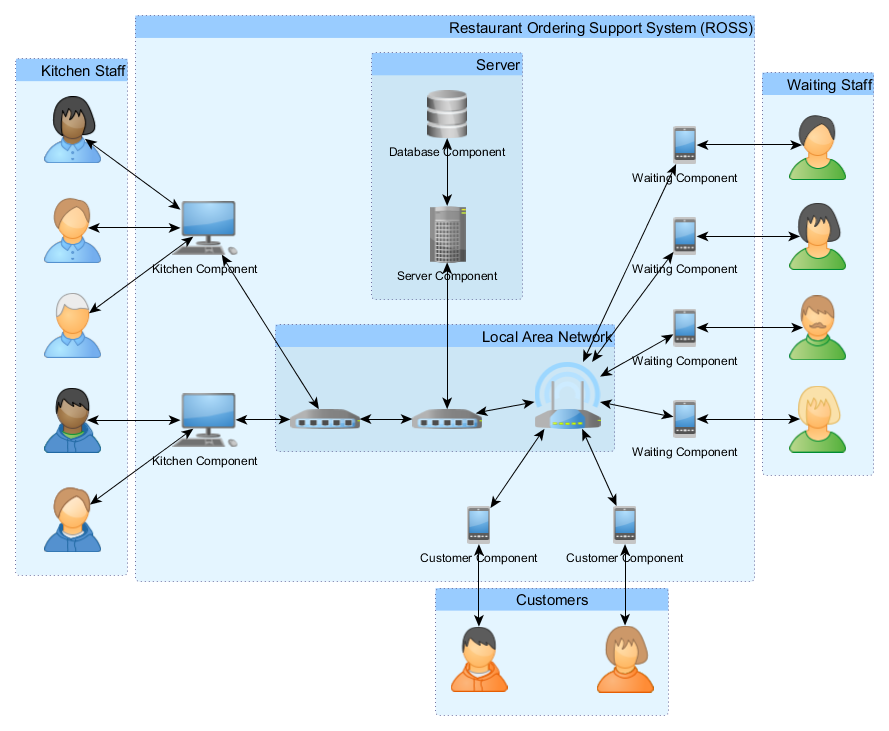
\includegraphics[scale=0.5]{Figures/SystemArchitectureDiagram.png}
\caption{Architectural overview of ROSS.}
\vspace{1cm}
\flushleft
As a web app, the exact number of devices and people connected to the Local Area Network is flexible.\\
No specification is made as to the Local Area Network topology.
\end{figure}

\pagebreak

\subsection{Existing software and infrastructure usage}

During the software development phase of the project, the software will be implemented on the existing LAMP server provided to students within the MACS department. This is to remove the need to implement and maintain a server to test on and allow us to focus on the web app itself. The same software stack would be utilised in the final product when installed within a restaurant, though not necessarily the same software versions.\\
This stack is chosen for its commonness and free open-source nature. This makes it cheap and easy to implement and maintain, especially when the client may not have a sizeable or experienced support system for web technologies.\\
\\
In terms of other software incorporated into the product, the decision has been made to use the React JavaScript library in order to ease the development of the User Interface (UI). The library makes it significantly easier to associate functionality and states with specific visual components, bringing JavaScript much closer to an object-orientated paradigm. The library also has functionality to react to changes in state and update the relevant UI elements, implementation specifics of which are not yet fully researched. No explicit plans are made to use any other libraries or frameworks not built-in to technologies used (e.g. the standard built-in PHP library). The project remains open to the potential offered by other libraries which may come up during development. These will be judged on, amongst other things, their ease of incorporation to the existing code base and any advantages they provide in the immediate and long-term future. Specific efforts will be made to avoid incorporating too many libraries and bloating the product with largely unused code.

\subsection{Development technologies}

Whilst each team member is to be allowed to use whatever development environment they desire, specific technologies will be used to facilitate cooperation.\\
\\
Git and GitHub will be used to provide strong version control and serve as a backup of all work, both complete and in progress. They also provide excellent tools to manage the integration of multiple peoples' work into a single cohesive unit.\\
\\
Documentation is primarily to be written using LaTeX to take full advantage of Git. Since Git cannot work with binary files (for example PDF, DocX), the fullness of its version control cannot be exploited unless a plain-text file format is used. LaTeX is written in plain text, allowing full use of version control. It also has the advantage of automating significant amounts of document formatting, making it easier to produce documentation in parallel and maintain a consistent aesthetic and format. It also makes the merging or documents easier.\\
\\
In terms of communication within the team, WhatsApp was decided as the method of choice. This is because email was felt too slow and easily missed, and of the various communication applications out there it was the one most members had in common. For more formal communication within the team and with external parties (such as line manager), email is used. This is because, although slower, email gives a clear record of communication both in attributing statements to people and specifying who received a given message.


\section{Definition of Terms} \label{subsec:Definitions}
\vspace{1cm}

\begin{tabulary}{1.2\textwidth}{l L}
Term & Definition \\ \midrule

LAMP & Stands for Linux, Apache, MySQL, PHP.\newline A typical, fully open-source software stack for web servers. \\ \midrule
MACS & Stands for Mathematical and Computer Sciences\newline The phrase "MACS department" is the common-usage name for the School of Mathematical and Computer Sciences within Heriot-Watt University. \\ \midrule
App & Abbreviation of application.
\end{tabulary}

\nocite{NoRisks}

\printbibliography
\end{document}